\subsection{Saturation effect to HEEP ID efficiency}
\label{HEEP_effect}
Here we use sample \texttt{/DoubleElectron\_FlatPt-300To6500/RunIISpring16DR80-\\PUFlat0to50\_80X\_mcRun2\_asymptotic\_2016\_v3-v1/AODSIM} to study the effect of saturation to HEEP ID efficiency.
The HEEP ID efficiency for saturated and unsaturated electron is shown in
Figure \ref{fig:HEEP_eff} and one can see the HEEP ID is safe for saturated
electron in endcap while for barrel it works well when the energy is lower than
around 3.2 TeV. The reason for the HEEP ID efficiency decrease quickly with energy for saturated electron in barrel is because of the showershape cut which can be seen in Figure \ref{fig:ShowerShape} and the efficiency of HEEP ID without showershape is shown in Figure \ref{fig:HEEP_noShower_eff}. The difference of the efficiency between saturated electron and unsaturated electron in Figure \ref{fig:HEEP_noShower_eff} in barrel is mainly from $\frac{H}{E}$ cut and in endcap it is mainly from EcalDriven cut.

\begin{figure}[bh]
  \begin{center}
    \begin{tabular}{cc}
      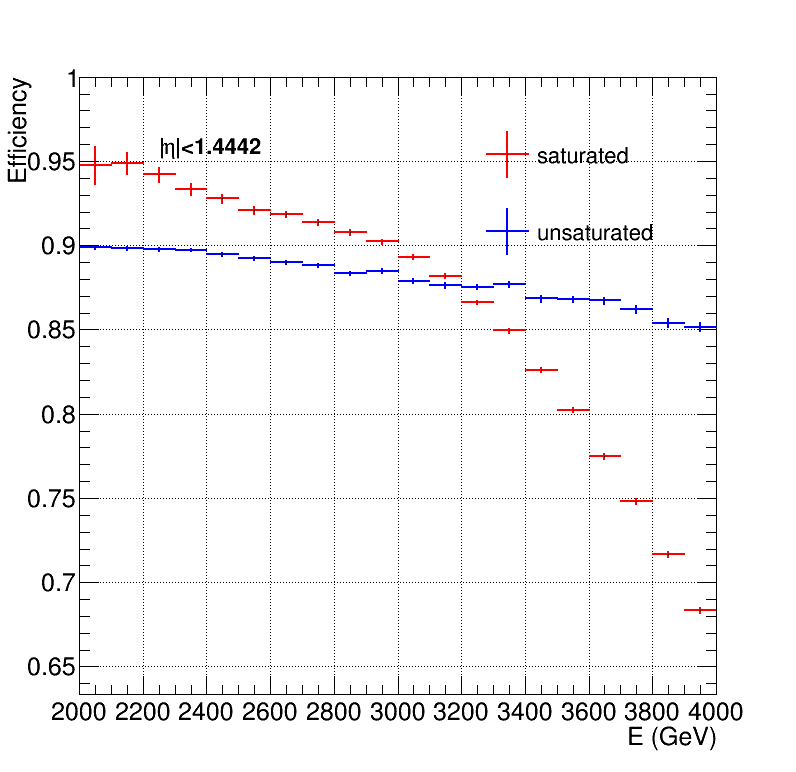
\includegraphics[width=0.45\textwidth]{chapters/Zprime/Saturation/images/FlatPt/compare_s_nos/nominal_HEEP_eff/compare_HEEP_eff_Barrel.png} &
      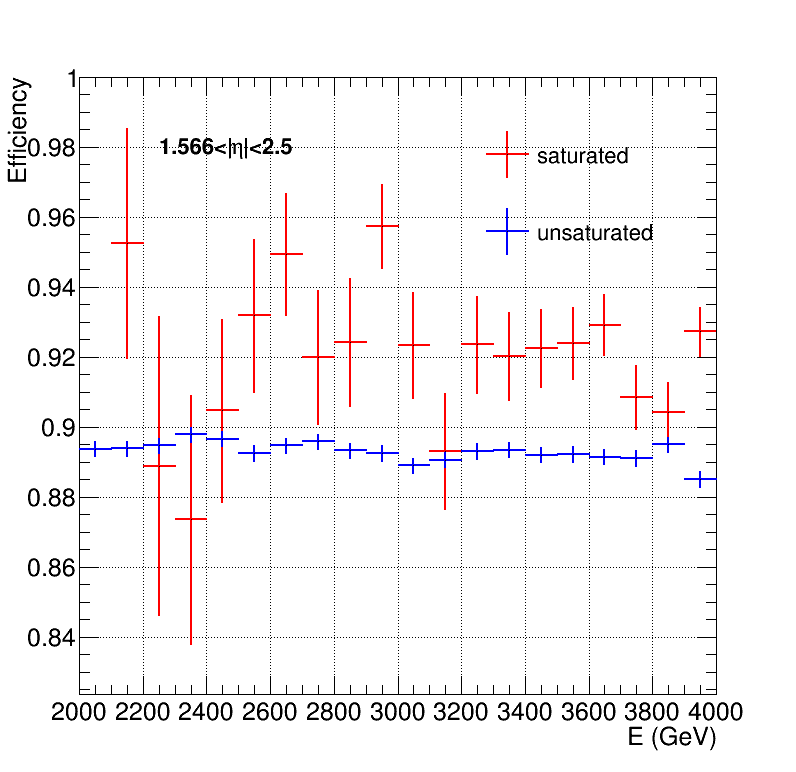
\includegraphics[width=0.45\textwidth]{chapters/Zprime/Saturation/images/FlatPt/compare_s_nos/nominal_HEEP_eff/compare_HEEP_eff_Endcap.png} \\
    \end{tabular}
    \caption{ The HEEP ID efficiency for saturated electron (red histogram) and unsaturated electron (blue histogram) for barrel (left) and endcap (right).}
    \label{fig:HEEP_eff}
  \end{center}
\end{figure}

\begin{figure}[bh]
  \begin{center}
    \begin{tabular}{cc}
      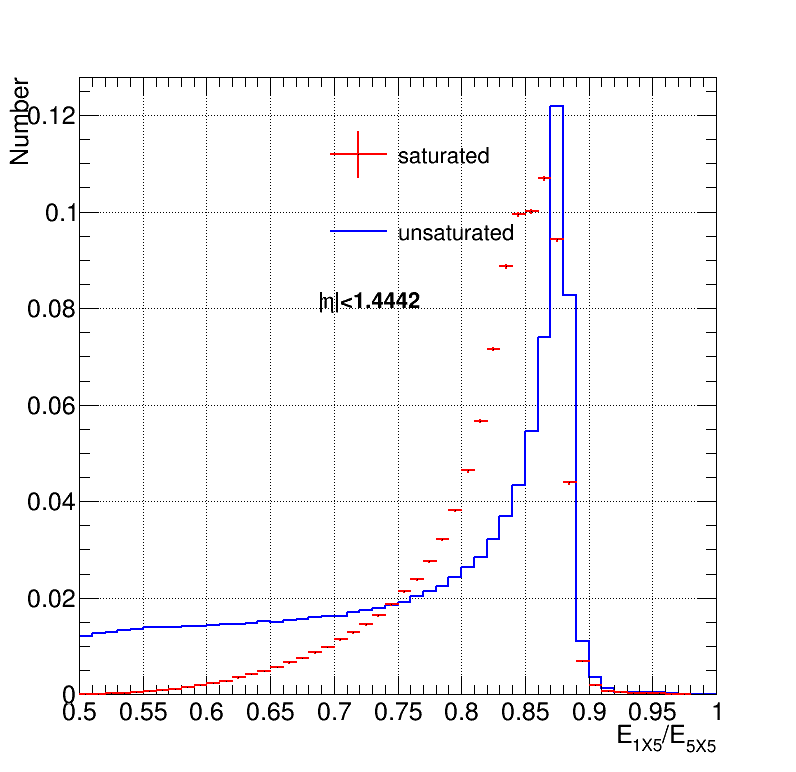
\includegraphics[width=0.45\textwidth]{chapters/Zprime/Saturation/images/FlatPt/compare_s_nos/compare_E15OverE55_Barrel.png} &
      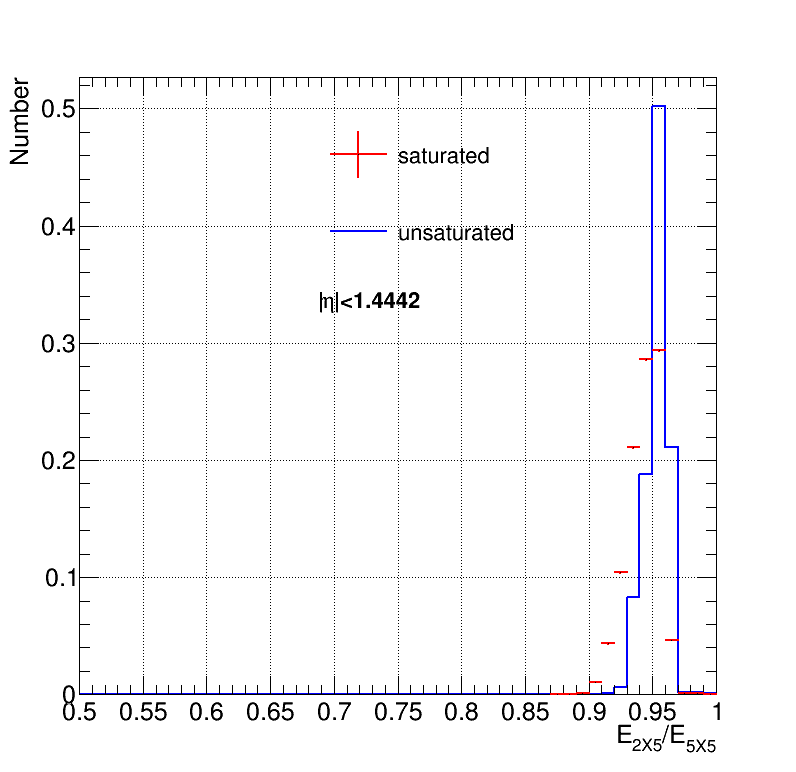
\includegraphics[width=0.45\textwidth]{chapters/Zprime/Saturation/images/FlatPt/compare_s_nos/compare_E25OverE55_Barrel.png} \\
      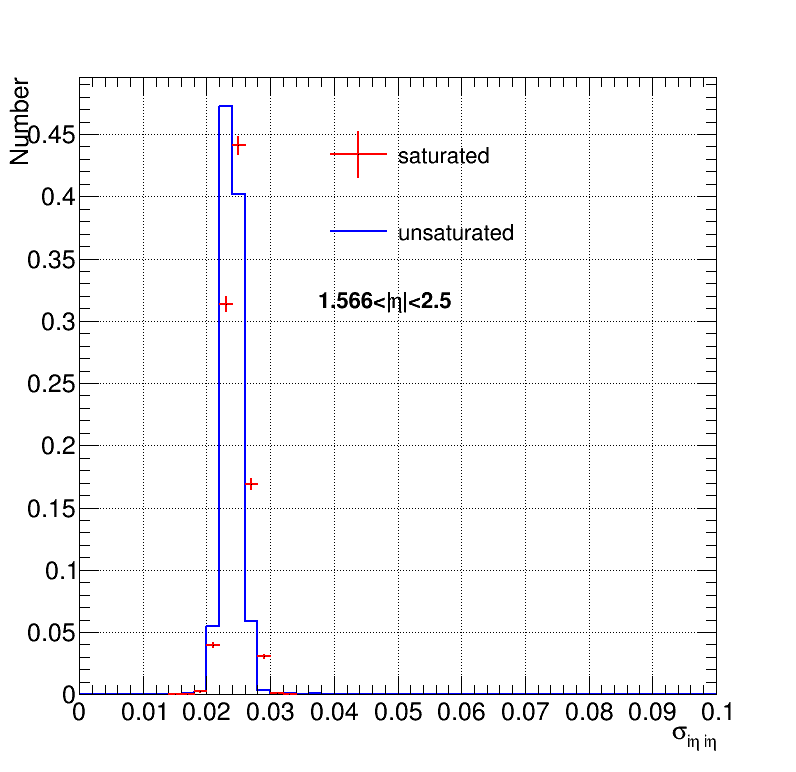
\includegraphics[width=0.45\textwidth]{chapters/Zprime/Saturation/images/FlatPt/compare_s_nos/compare_Sieie_Endcap.png} &
    \end{tabular}
    \caption{ The distributions of the value of HEEP ID showershape variables for barrel (top) and endcap (bottom) for saturated (red histogram) and unsaturated (blue histogram) electrons.}
    \label{fig:ShowerShape}
  \end{center}
\end{figure}


\begin{figure}[bh]
  \begin{center}
    \begin{tabular}{cc}
      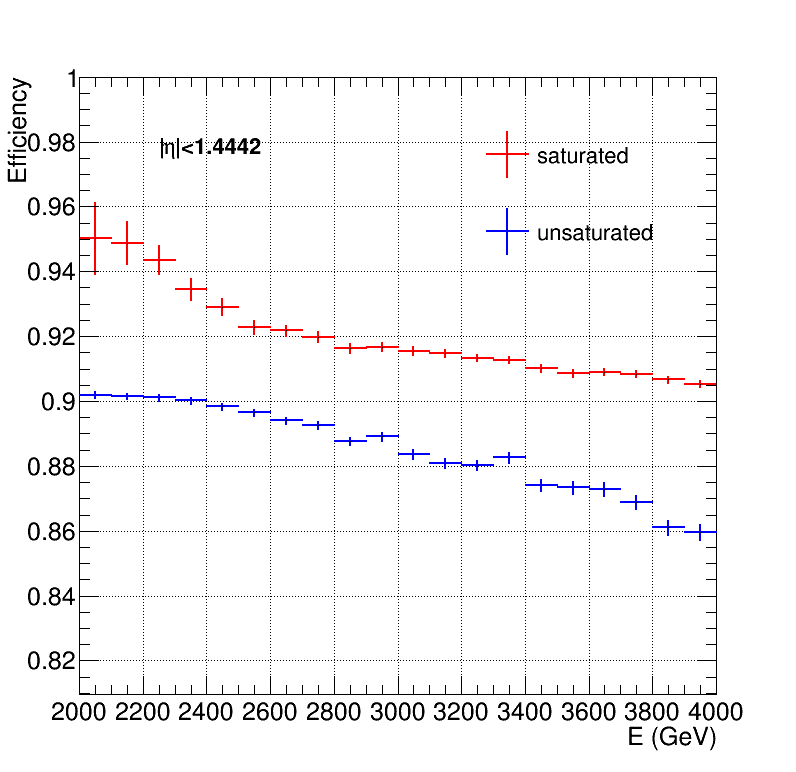
\includegraphics[width=0.45\textwidth]{chapters/Zprime/Saturation/images/FlatPt/compare_s_nos/noShowerShape_HEEP_eff/compare_HEEP_eff_Barrel.png} &
      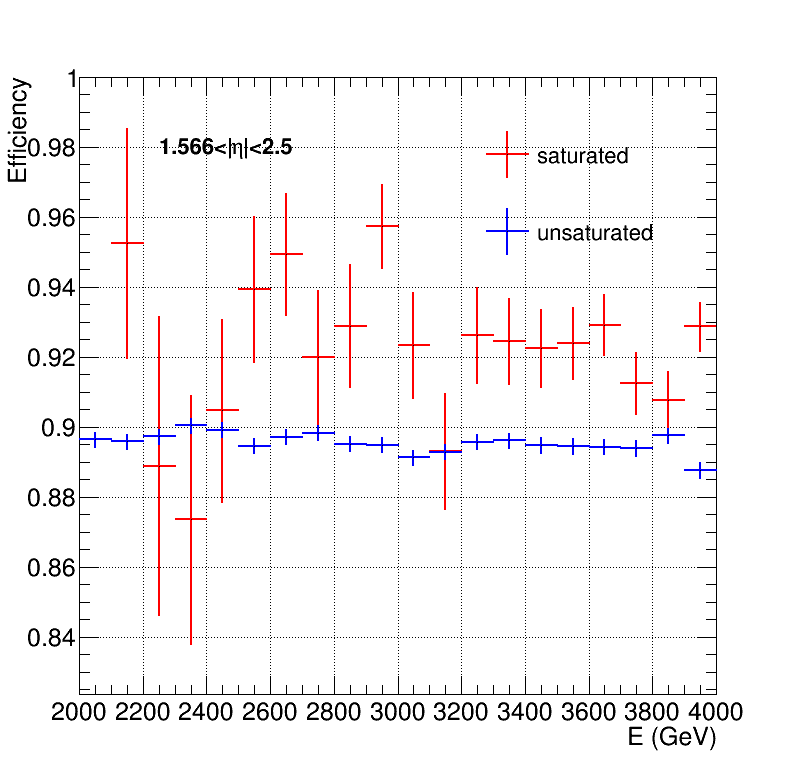
\includegraphics[width=0.45\textwidth]{chapters/Zprime/Saturation/images/FlatPt/compare_s_nos/noShowerShape_HEEP_eff/compare_HEEP_eff_Endcap.png} \\
    \end{tabular}
    \caption{ The HEEP ID without showershape criteria efficiency for saturated (red histogram) and unsaturated electrons (blue histogram) for barrel (left) and endcap (right).}
    \label{fig:HEEP_noShower_eff}
  \end{center}
\end{figure}
